%!TEX program = xelatex

\documentclass[compress]{beamer}
%--------------------------------------------------------------------------
% Common packages
%--------------------------------------------------------------------------

\definecolor{links}{HTML}{663000}
\hypersetup{colorlinks,linkcolor=,urlcolor=links}

\usepackage[english]{babel}
\usepackage{pgfpages} % required for notes on second screen
\usepackage{graphicx}

\usepackage{multicol}


\usepackage{tabularx,ragged2e}
\usepackage{booktabs}

\setlength{\emergencystretch}{3em}  % prevent overfull lines
\providecommand{\tightlist}{%
  \setlength{\itemsep}{0pt}\setlength{\parskip}{0pt}}


\usetheme{hri}

\usepackage{remreset}% tiny package containing just the \@removefromreset command
\makeatletter
\@removefromreset{subsection}{section}
\makeatother
\setcounter{subsection}{1}

\newcommand{\source}[2]{{\tiny\it Source: \href{#1}{#2}}}

\usepackage{tikz}
\usetikzlibrary{mindmap,backgrounds,positioning}

\graphicspath{{part1/figs/}}

\title{ROCO222 \newline Introduction to Sensors and Actuators}
\subtitle{Part 1 -- Introduction}
\date{}
\author{Séverin Lemaignan}
\institute{Centre for Neural Systems and Robotics\\{\bf Plymouth University}}

\begin{document}

\licenseframe{github.com/severin-lemaignan/module-introduction-sensors-actuators}

\maketitle

\begin{frame}{Who am I?}
    I am Dr. Séverin Lemaignan. My office is B316 Portland Square
\end{frame}

\begin{frame}{And what do I do?}

\begin{multicols}{2}

    \textbf{Cognitive robotics}

  Building robots and their artificial intelligence inspired on natural
  systems, such as developing children

    \textbf{Human-Robot Interaction}

  Building robots that can work alongside people, using social cues that
  people use to communicate

    \begin{center}
        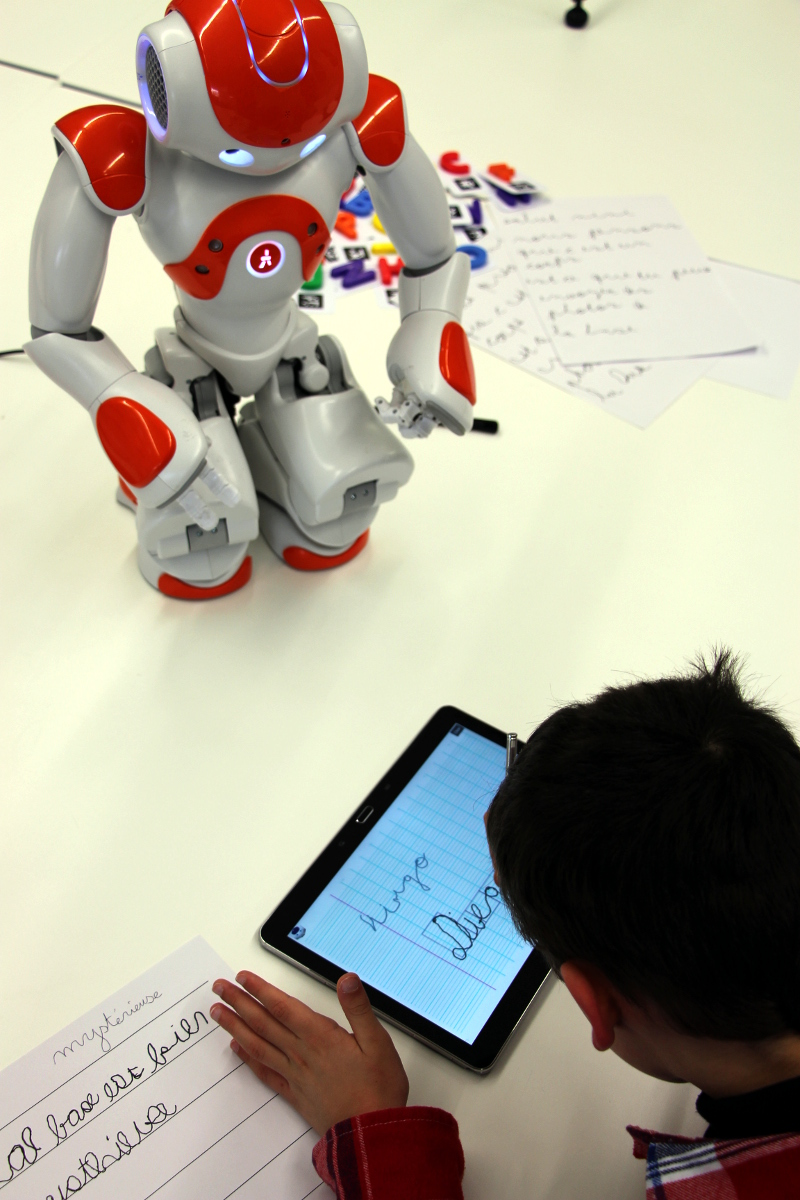
\includegraphics[width=0.8\linewidth]{cowriter}
    \end{center}

\end{multicols}
\end{frame}

\begin{frame}{Availability}

    \begin{itemize}
        \item I have lots of time (2 hours) to deal with your queries in the laboratory sessions
        \item  Otherwise, the best thing to do is to email me first and see if I can sort out your query. If not then I will arrange a time to meet up with you.
        \item Don't forget – if you have any problems, or even if you are not sure about something - just email me

    \end{itemize}

    \begin{center}
        severin.lemaignan@plymouth.ac.uk
    \end{center}
\end{frame}

\begin{frame}{Registration}
        \centering
        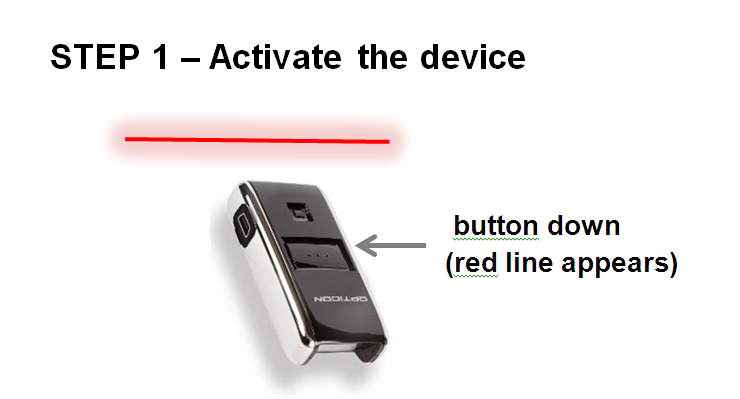
\includegraphics[width=0.4\linewidth]{registration1}
        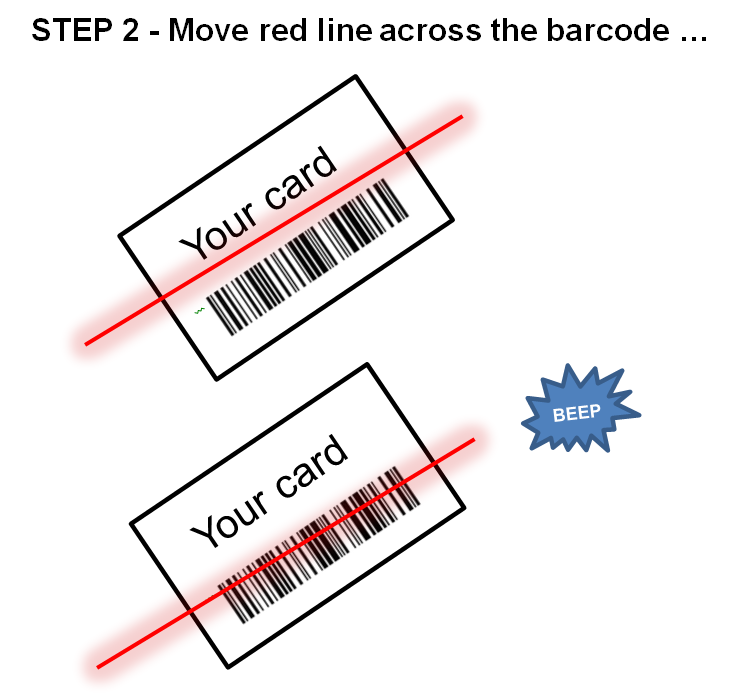
\includegraphics[width=0.4\linewidth]{registration2}
\end{frame}

\begin{frame}{Special needs}

    \begin{itemize}

    \item Anyone with dyslexia or any other special needs that requires any form
        of support during examinations and tests should email me immediately.

    \item Please do not ASSUME that I know of your condition. It takes the
        University some weeks to process data and forward it to the correct
            members of staff.

    \item Even if you are currently undergoing assessment, it is advisable to
        contact me and I will organize suitable support for you during your
            tests and exams.

    \item Contact me if any issues relating to harassment, inclusivity or if
        language/cultural difficulties arise.

    \end{itemize}
\end{frame}

\begin{frame}{Labs}
    \begin{itemize}
        \item ROCO222 is also taught and supervised in a computer laboratory for
            a TWO HOURS EACH WEEK.
        \item There are 2 labs so please go to your timetabled group and pair up
            with someone
    \end{itemize}

    \centering
          \begin{tabular}{@{}llll@{}}
                \toprule
                Day?                & Time? & Where?   & Who? \\ \midrule
                Monday -- Lab T1/\textbf{01} & ?     & SMB 307  & ? \& myself            \\
                Friday -- Lab T1/\textbf{02} & ?     & SMB 307  & ? \& myself          \\ \bottomrule
            \end{tabular}


\end{frame}

\section{Assessment}

\begin{frame}{Assessment}
    \begin{exampleblock}{Formative vs Summative}
        \textbf{Formative}: during the term; \textbf{Summative}: at the end of
        the term.
    \end{exampleblock}

    \begin{itemize}
        \item There will be practical assessments in the form of laboratory
            practical work (60\%)
        \item First practical needs to be submitted by 12:00, 17th October 2016
            TODO: update date
        \item Feedback within 20 working days
        \item Complete lab journal submitted Thursday 4pm, 12th January 2017
            TODO: update date
        \item There will be a final written exam (40\%) -- \textbf{note that the
            exam questions may be on material discussed during the labs}
    \end{itemize}

\end{frame}


\section{Robotics: what are your expectations?}

\imageframe[color=black, caption=github.com/severin-lemaignan/module-introduction-sensors-actuators]{github}

\section{Module Overview}

\videoframe[0.56]{part1/figs/NISSAN-ProPILOT-chair.mp4}


\begin{frame}{Module aims}
    \begin{itemize}
        \item<+-> Develop an in-depth understanding of what electical motors are,
            how the work (hands-on!), how they are characterised
        \item<+-> Learn how to control them, and program an embedded controller
            for your own motor
        \item<+-> Get a first hand-on experience with a complete robotic system:
            from the hardware, to the low-level closed-loop control, to
            system-level visualisation
    \end{itemize}
\end{frame}

\begin{frame}{Learning outcomes}
    \begin{enumerate}
        \item<+-> Demonstrate knowledge and critical understanding of the operating
            \textbf{characteristics of electrical motors} (brush, brushless,
            servo, stepper motors)
        \item<+-> Comprehend and characterise the effects of \textbf{closing the speed and current
            loops} in drive systems; demonstrate it practically by \textbf{creating a
            closed loop motor system}
        \item<+-> Understand the fundamentals of the \textbf{ROS middleware}, and use it for
            simple robot visualisations
        \item<+-> Feel confident when using the \textbf{Linux command-line}
        \item<+-> Know how to use and reflect on \textbf{document/code versioning and
            sharing} (with git)
    \end{enumerate}
\end{frame}

\begin{frame}{In your curriculum...}
    \begin{itemize}
        \item Lat year: TODO control?
        \item Next term: \textbf{ROCO224} -- TODO
        \item Next year: \textbf{ROCO318} -- sensors, algorithms, kinematics, AI (path
            planning, localisation)
    \end{itemize}
\end{frame}

\begin{frame}{This module: syllabus}

\begin{itemize}
    \item<+-> DC motors, brushed \& brushless
    \item<+-> the physics behind it (electromagnetics)
    \item<+-> servo-motors, stepper motors
    \item<+-> closed-loop motor control, PWM, PID, H-bridge
    \item<+-> the ROS middleware, joint state, kinematics 101, visualisation
    \item<+-> mechanical design principles \& mechanical components
\end{itemize}

\end{frame}

\section{Laboratory Coursework}

\begin{frame}{Lab journal \& Command-line 101}
    \begin{itemize}
        \item Document versioning: what is GIT?
        \item Creating \& managing a lab journal with GIT and markdown
        \item Linux command-line
        \item Compiling and running code
        \item How to keep organised!
    \end{itemize}
\end{frame}

\begin{frame}{Build a simple DC motor}
    \begin{columns}
        \begin{column}{0.45\linewidth}
            Build a DC brushed motor from first principles
            \begin{itemize}

                \item Wind armature

                \item Position field magnets

                \item Build commutator

                \item Test operation

                \item Measure characteristics

            \end{itemize}

        \end{column}
        \begin{column}{0.45\linewidth}

            \begin{center}
                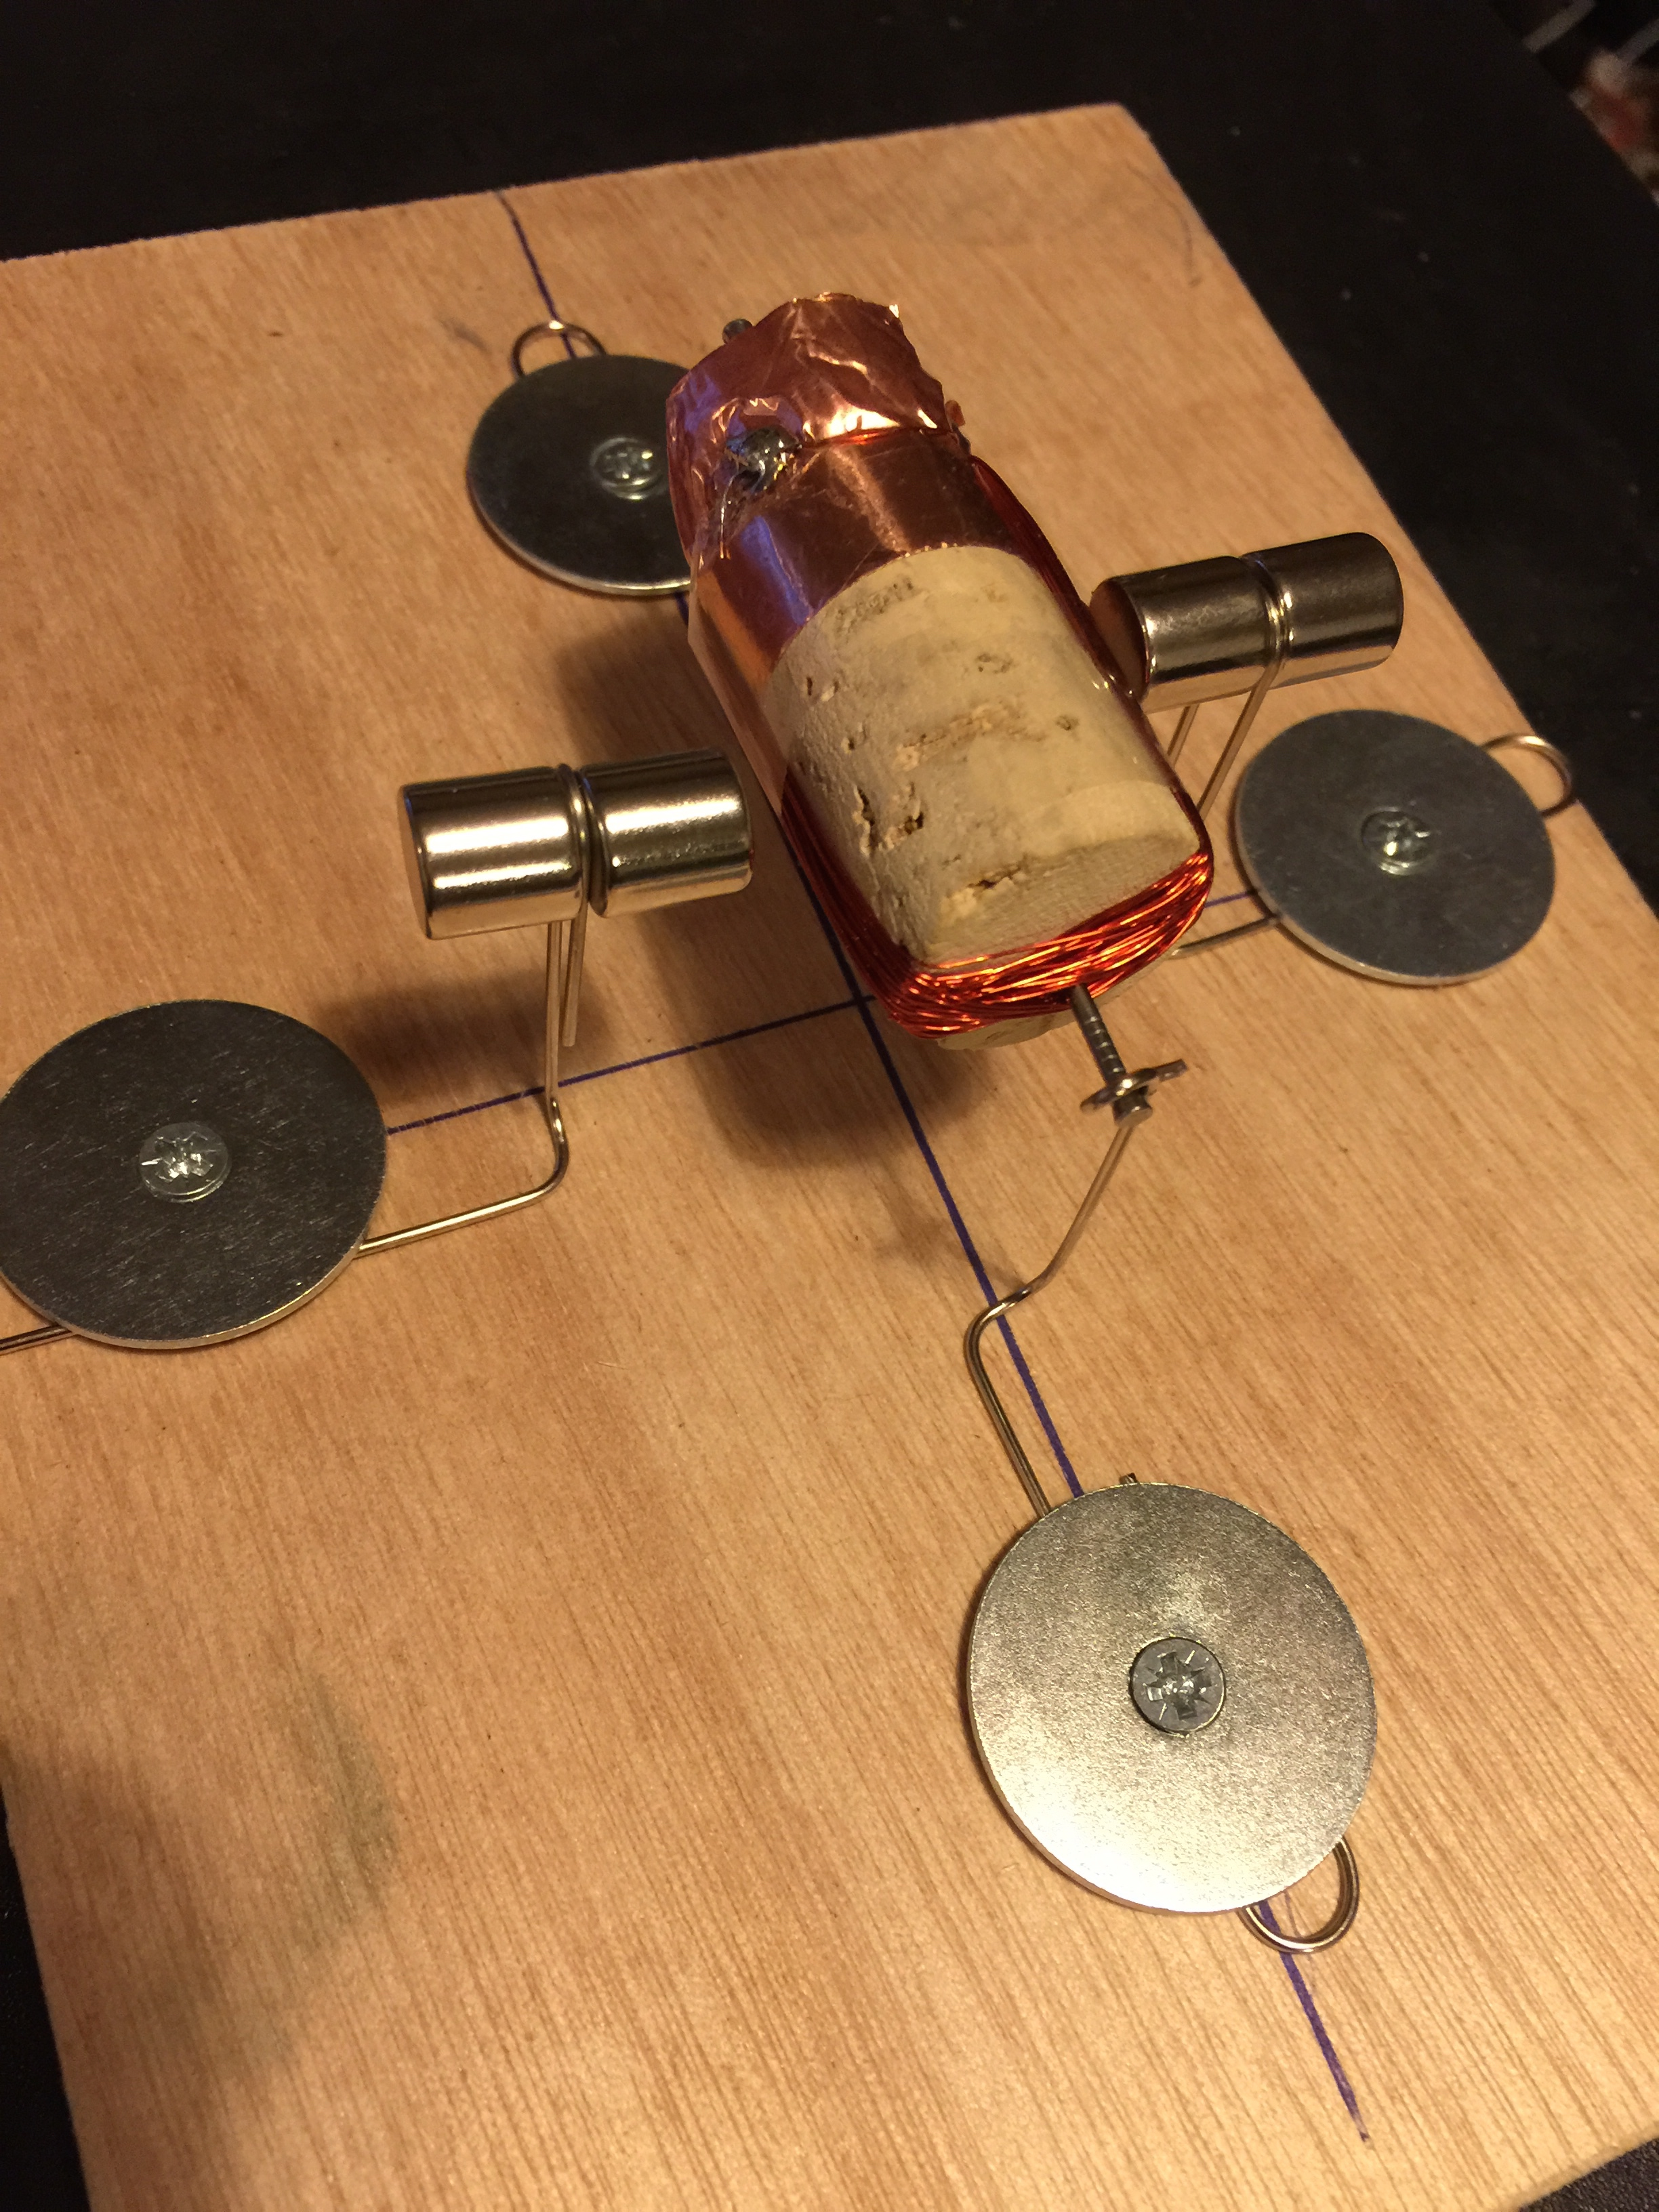
\includegraphics[width=0.8\columnwidth]{simple-dc-motor}\\
                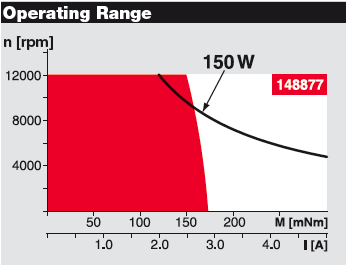
\includegraphics[width=0.8\columnwidth]{motor-characterisation}
            \end{center}

        \end{column}
    \end{columns}
\end{frame}

\begin{frame}{Introduction to Arduino and simple motor control}
    \begin{columns}
        \begin{column}{0.45\linewidth}

            \begin{itemize}
                \item Controlling a DC motor using an Arduino
                \item Build a speed-controlled electric fan \eg use
                    temperature sensor

                \item Control an RC servo using an Arduino
            \end{itemize}
        \end{column}
        \begin{column}{0.45\linewidth}

            \begin{center}
                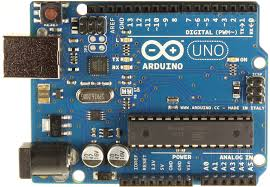
\includegraphics[width=0.8\columnwidth]{arduino}\\
                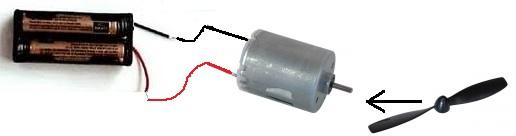
\includegraphics[width=0.8\columnwidth]{dc-motor-fan}\\
                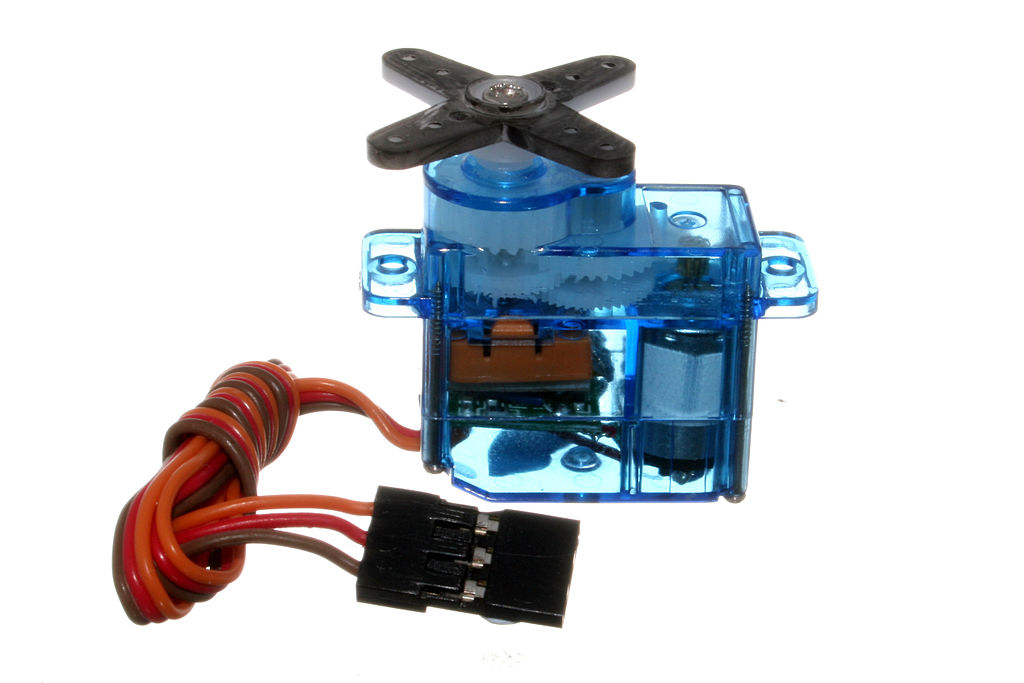
\includegraphics[width=0.8\columnwidth]{servo}\\
            \end{center}

        \end{column}
    \end{columns}
\end{frame}


\begin{frame}{Attention: weeks off}
    TODO Do I tell them now? I might be able to find someone to replace me
    (Martin for instance)
\end{frame}

%%%%%%%%%%%%%%%%%%%%%%%%%%%%%%%%%%%%%%%%%%%%%%%%%%%%%%%%%%%%%%%%%%%%%%%

\begin{frame}{}
    \begin{center}
        \Large
        That's all, folks!\\[2em]
        \normalsize
        Questions:\\
        Portland Square B316 or \url{severin.lemaignan@plymouth.ac.uk} \\[1em]

        Slides:\\
        \href{https://github.com/severin-lemaignan/module-mobile-and-humanoid-robots}{\small
        github.com/severin-lemaignan/module-introduction-sensors-actuators}

    \end{center}
\end{frame}



\end{document}
